\chapter{Other deconvolution}
\section{Product-SRP-PHAT}
A simple deconvolution approach could be to penalize sources which are only detected by a subset of the microphone pair combinations. This could be done by taking a product and not a sum in Eq. \ref{eq:srpSumInd}.
\begin{equation}
    S_{SRP}(\theta,\phi)=\prod\limits_{i=1}^{M-1}{R_{x_0,x_i}[f_{0,i}(\theta,\phi)]}
     \label{eq:srpProdInd}
\end{equation}
This way, if a peak is caused by a single localization circle, the cross-correlation values from other microphone pairs would be close to zero, and thus would scale the false peak down. The localization results from this are given in fig. \ref{fig:4mic1srcNoisyProd}.
\begin{figure}[!ht]
    \centering
    \begin{subfigure}[b]{0.96\textwidth}
    \centering
    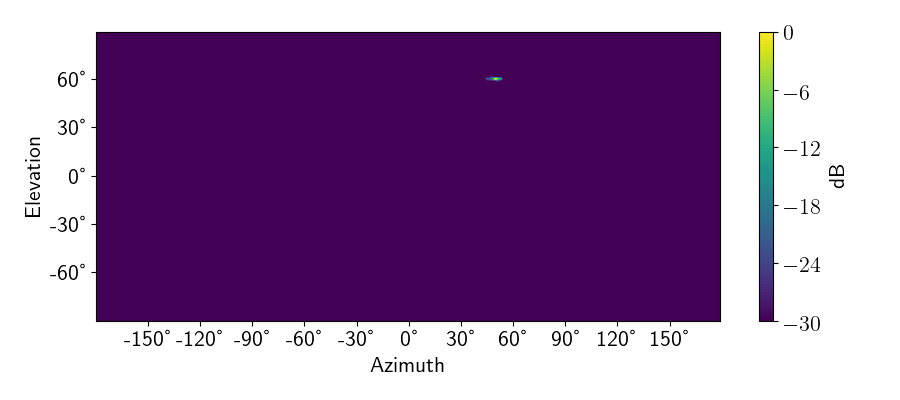
\includegraphics[width=0.8\textwidth]{Figures/Ind4mic1srcProd20.png}
\end{subfigure}
\vskip \baselineskip
\begin{subfigure}[b]{0.96\textwidth}
    \centering
    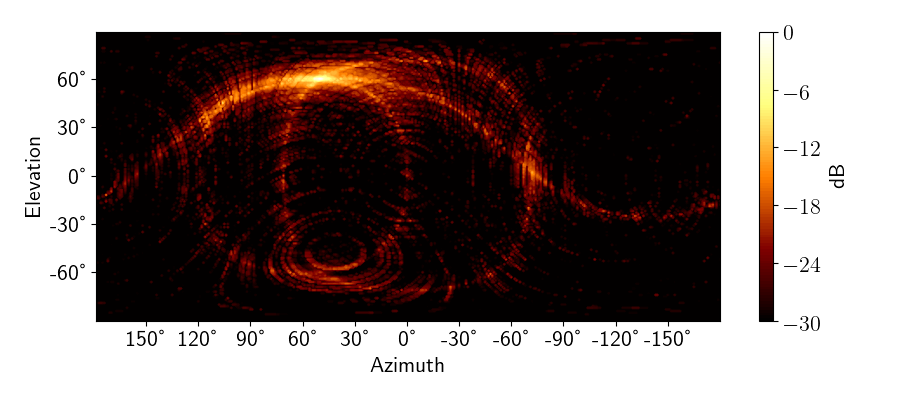
\includegraphics[width=0.8\textwidth]{Figures/Ind4mic1srcProd0.png}
\end{subfigure}
\vskip \baselineskip
\begin{subfigure}[b]{0.96\textwidth}
    \centering
    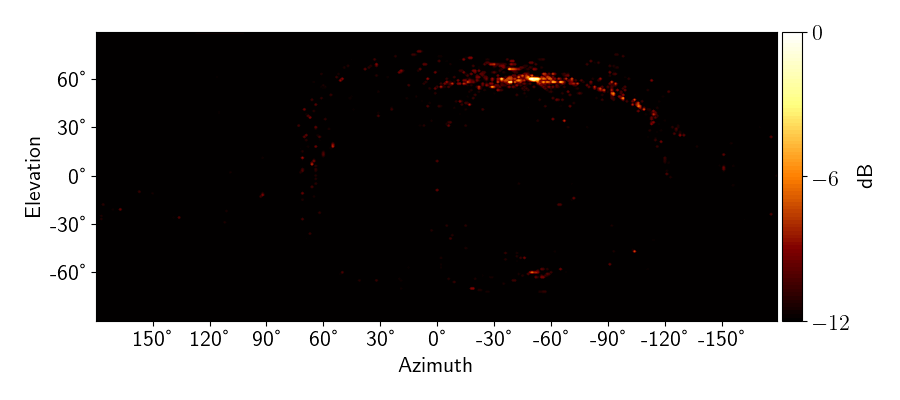
\includegraphics[width=0.8\textwidth]{Figures/Ind4mic1srcProdNeg10.png}
\end{subfigure}
\caption{Figures depict from top-to-bottom product-SRP-PHAT localization results  with SNR = 20dB, SNR = 0dB, SNR = -10dB}
\label{fig:4mic1srcNoisyProd}
\end{figure}
\newpage
The drawback of using product-SRP-PHAT is that the sound level difference between the different sound sources is lost. In normal SRP-PHAT, the array magnitude response at a particular azimuth and elevation is averaged over all microphone pair combinations. Then the level difference between 2 sources is maintained. In product-SRP-PHAT this would not be the case. However if it is assumed that a particular source will have similar magnitude response for all microphone pairs (which is not a strong assumption in far-field), then taking source power $P_{SRP}={S_{SRP}}^{1/M}$, the level difference can be maintained.  Fig. \ref{fig:4mic2srcNoisyCompare} depicts the results of product-SRP-PHAT after level correction.
\begin{figure}[!ht]
    \centering
    \begin{subfigure}[b]{0.96\textwidth}
    \centering
    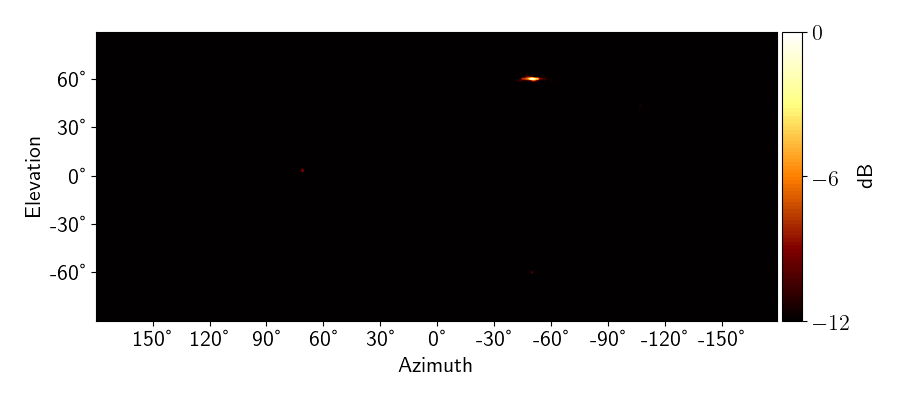
\includegraphics[width=0.8\textwidth]{Figures/Ind4mic1srcProd20Corr.png}
\end{subfigure}
\vskip \baselineskip
\begin{subfigure}[b]{0.96\textwidth}
    \centering
    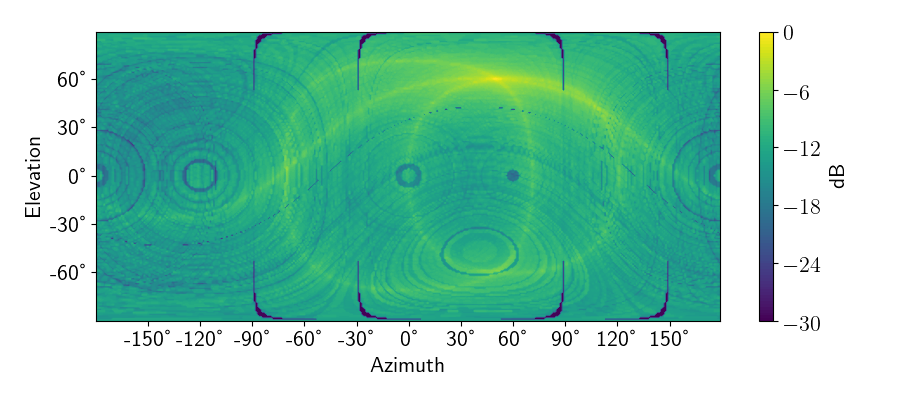
\includegraphics[width=0.8\textwidth]{Figures/Ind4mic1srcProd0Corr.png}
\end{subfigure}
\vskip \baselineskip
\begin{subfigure}[b]{0.96\textwidth}
    \centering
    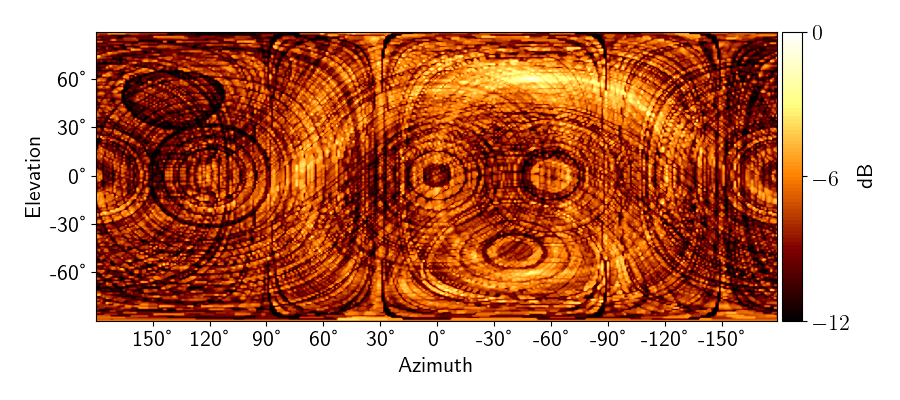
\includegraphics[width=0.8\textwidth]{Figures//Ind4mic1srcProdNeg10Corr.png}
\end{subfigure}
\caption{Figures depict from top-to-bottom level corrected product-SRP-PHAT localization results with SNR = 20dB, SNR = 0dB, SNR = -10dB}
\label{fig:4mic2srcNoisyCompare}
\end{figure}

\section{Threshold SRP-PHAT}
For product SRP-PHAT, if one of the cones is really high is magnitude, the algorithm might not be able to penalize a wrong location enough by simple multiplication with low power from other microphone pairs. This means that if one of the microphone pairs detects a very low power at a particular location, it should have a higher priority when deciding the power at that location. One way to achieve this could be to sort the power for the different cones at each location, and then divide the values with each other. If the numbers are quite different in magnitude, the division could then cross a certain pre-defined threshold, and the power at that location could be set to zero. However, while this methodology could work for a single source, for multiple sources playing at different levels, and which share a localization cone, this would lead to the masking of the lower magnitude source.   